%% sections/methodology.tex
\section{Methodology}
\label{sec:method}

This section describes the computational architecture, the core
algorithms, and the design choices that make the system reproducible,
extensible, and suitable for controlled experimentation.

\subsection{System architecture}

The runtime is organised into four groups
(Figure~\ref{fig:arch}), matching the Architecture tab in the live
application.  Data flows strictly downward: the market substrate
feeds the utility-agent pipeline, which routes through the matching
engine into the append-only logger.

\begin{figure}[H]
\centering
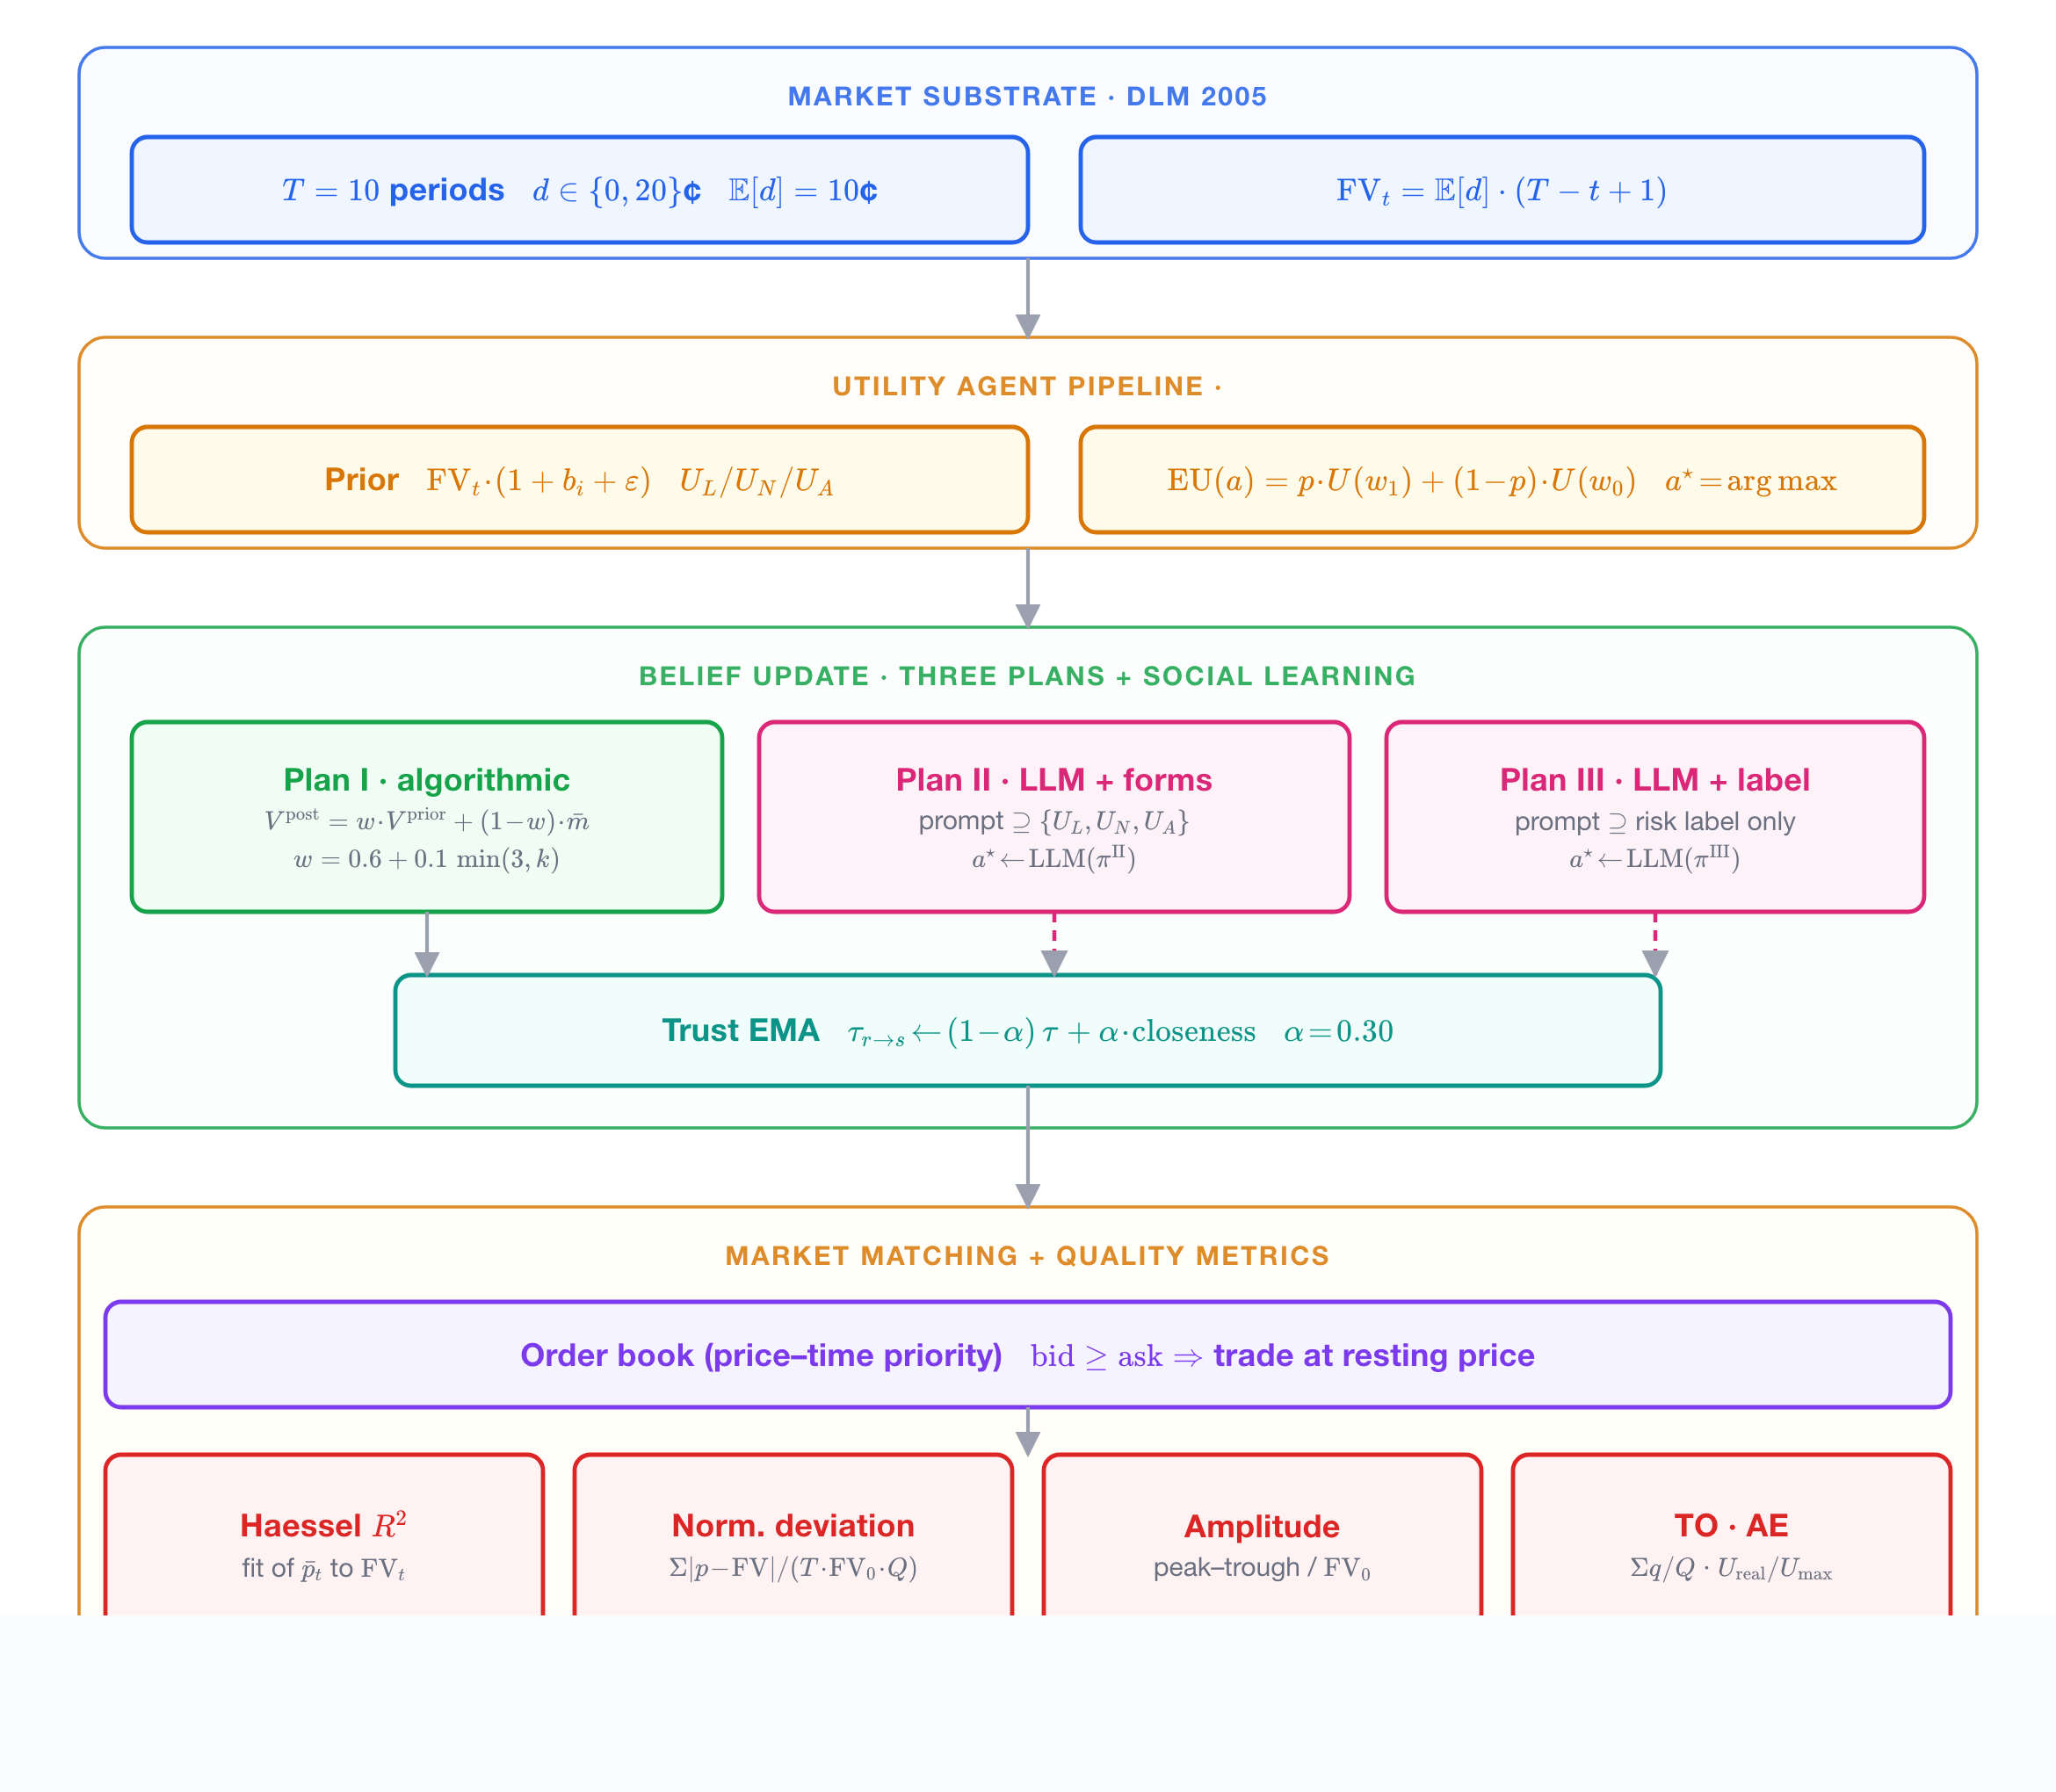
\includegraphics[width=\columnwidth]{figures/arch.png}
\caption{Mathematical architecture, mirroring the live Architecture
tab.  Four groups: the DLM market substrate feeds into the
six-agent utility pipeline; Plan~I evaluates EU algorithmically,
Plans~II/III (dashed) substitute a direct LLM action selection
from the seven-element action set.  All paths converge at the
matching engine and quality metrics.}
\label{fig:arch}
\end{figure}

\emph{Market substrate.}  The DLM~2005 dividend process and the
continuous double auction with price-time priority order book.
Fundamental value $\FV_t = \mu(T{-}t{+}1)$ resets at every round
boundary.

\emph{Utility-agent pipeline.}  Six agents carry persistent bias
$b_i$, risk preference ($U_L$/$U_N$/$U_A$), and experience counter
$k_i$.  Each period boundary triggers a belief update---Plan~I
blends the prior with peer claims; Plans~II/III substitute an LLM
call---followed by expected-utility scoring over the action set
$\{\text{hold, bid, ask}\}$.

\emph{LLM belief update.}  A pluggable oracle that operates outside
the deterministic core.  Plan~II prompts include the closed-form
utility expression; Plan~III names only the risk label.  The
consume-and-cache pattern (Algorithm~\ref{alg:belief}) ensures the
tick loop never blocks on network latency.

\emph{Market matching and metrics.}  The matching engine settles
fills at the resting price.  An append-only logger records traces,
snapshots, and events; no entry is ever mutated, which is the
invariant that enables exact replay.  Quality metrics ($R^2_H$,
ND, amplitude, turnover, allocative efficiency) are computed from
the logged history.

\subsection{Tick-level simulation loop}

Algorithm~\ref{alg:tick} specifies one tick of the simulation.  The
engine runs 720 ticks per session ($R{\times}T{\times}K =
4{\times}10{\times}18$).

\begin{algorithm}[h]
\caption{Tick-level simulation step}
\label{alg:tick}
\begin{algorithmic}[1]
\State $\text{tick} \gets \text{tick} + 1$
\State $\sigma \gets \text{FisherYates}(\text{agentIds},\;\text{rng})$
  \Comment{seeded shuffle}
\For{$i \in \sigma$}
  \State $a_i \gets \text{agent}_i.\text{decide}(\text{market},
    \text{rng}, \text{ctx})$
  \If{$a_i.\text{type} \in \{\text{bid},\text{ask}\}$}
    \State $o \gets \text{Order}(a_i)$
    \State $\text{fills} \gets \text{market.submit}(o)$
      \Comment{match at resting price}
    \ForAll{fill $f \in \text{fills}$}
      \State buyer.cash $\mathrel{-}= f.\text{price}$;\;
             buyer.inv $\mathrel{+}= 1$
      \State seller.cash $\mathrel{+}= f.\text{price}$;\;
             seller.inv $\mathrel{-}= 1$
    \EndFor
  \EndIf
  \State logger.trace($i$, $a_i$)
\EndFor
\State market.priceHistory.append(tick, period, round, lastPrice,
  $\FV_t$)
\end{algorithmic}
\end{algorithm}

The Fisher-Yates shuffle on line~2 consumes $N{-}1$ draws from the
seeded PRNG and determines the evaluation order for the tick.  Order
submission on line~7 invokes the matching engine, which walks the
opposite side of the book until no crossing remains or the order is
exhausted.  Self-match prevention cancels any resting order belonging
to the submitting agent before attempting a fill.

\subsection{Period-boundary protocol}

Algorithm~\ref{alg:period} specifies the operations at every period
boundary (every $K{=}18$ ticks).

\begin{algorithm}[h]
\caption{Period-boundary protocol}
\label{alg:period}
\begin{algorithmic}[1]
\State Withdraw all outstanding orders from the book
\State $d \gets \text{rng}() < 0.5\;?\;0\;:\;2\mu$
  \Comment{dividend draw}
\ForAll{agent $i$ with inventory${}>0$}
  \State $\text{cash}_i \mathrel{+}= d \times \text{inv}_i$
\EndFor
\If{utility agents present}
  \ForAll{utility agent $i$}
    \State $i.\text{communicate}()$
      \Comment{broadcast $\hat v_i$ per eq.~\eqref{eq:trust}}
  \EndFor
  \State trustTracker.update(messageBus, market, $\alpha$)
  \If{plan $\in$ \{II, III\}}
    \State Fire async LLM batch; cache replies in llmBeliefs
  \EndIf
  \ForAll{utility agent $i$}
    \State $V_i^{\text{post}} \gets
      \text{updateBelief}_{\text{plan}}(i,\;\text{ctx})$
      \Comment{Alg.~\ref{alg:belief}}
  \EndFor
\EndIf
\end{algorithmic}
\end{algorithm}

\subsection{Belief-update dispatch}

The belief-update step is the single point in the pipeline where the
three plans diverge.  Algorithm~\ref{alg:belief} specifies the
dispatch.

\begin{algorithm}[h]
\caption{Decision dispatch for agent $i$}
\label{alg:belief}
\begin{algorithmic}[1]
\If{llmActions[$i$] exists}
  \Comment{Plan II or III succeeded}
  \State $a_i^\star \gets \text{translateAction}(\text{llmActions}[i])$;\;
    clear slot
  \Comment{consume LLM action}
  \If{$a_i^\star$ is valid}
    \State \Return $a_i^\star$
  \EndIf
\EndIf
\State \Comment{Plan I EU evaluation, or fallback from II/III}
\State $w \gets 0.6 + 0.1\,\min(3,\;k_i)$
  \Comment{experience weight}
\State $\msgs_i \gets$ foreign peer claims this period
\If{$|\msgs_i| > 0$}
  \State $V_i^{\text{post}} \gets w \cdot \FV_t +
    (1{-}w)\cdot\overline{\msgs}_i$
\Else
  \State $V_i^{\text{post}} \gets \FV_t$
\EndIf
\State $V_i^{\text{prior}} \gets V_i^{\text{post}}$
  \Comment{carry forward to next period}
\end{algorithmic}
\end{algorithm}

The consume-and-translate pattern (lines~1--5) is central to the
design.  The LLM call is fired asynchronously at the \emph{previous}
period boundary (Algorithm~\ref{alg:period}, line~12); the result is
read synchronously at the \emph{current} period boundary.  If the
call has not returned or the action is invalid, the agent falls
through to Plan~I's EU evaluation (lines~6--13).  The LLM returns
one of seven discrete actions: \texttt{BUY\_NOW}, \texttt{SELL\_NOW},
\texttt{BID\_1}, \texttt{BID\_3}, \texttt{ASK\_1}, \texttt{ASK\_3},
or \texttt{HOLD}; \texttt{translateAction} maps these to orders
using the current book state.  This architecture has three
consequences.
\emph{First}, the tick loop never blocks on network latency.
\emph{Second}, Plan~I is the exact counterfactual for any LLM
experiment: a failed action produces the same decision as the
algorithmic EU evaluation.
\emph{Third}, every session can be replayed offline, since the
fallback path is fully deterministic under the seeded PRNG.

\subsection{Round-boundary protocol}

Algorithm~\ref{alg:round} specifies the operations at the end of
period~$T$ of every non-final round.

\begin{algorithm}[h]
\caption{Round-boundary protocol (end of period $T$, round $r < R$)}
\label{alg:round}
\begin{algorithmic}[1]
\ForAll{agent $i$}
  \State roundFinalCash[$r$][$i$] $\gets$ cash$_i$
    \Comment{payoff ledger}
\EndFor
\ForAll{agent $i$}
  \State $k_i \gets k_i + 1$
    \Comment{increment experience}
\EndFor
\If{strictDLM \textbf{and} $r = 3$}
  \State Select $k \in \{2,4\}$ agents by Fisher-Yates
  \State Replace with fresh agents ($k_i{=}0$, iid endowment)
    \Comment{T2 or T4}
\EndIf
\ForAll{agent $i$}
  \State cash$_i \gets$ spec$_i$.cash;\;
    inv$_i \gets$ spec$_i$.inventory
    \Comment{rewind}
\EndFor
\State Clear order book; null lastPrice
\State round $\gets r{+}1$;\; period $\gets 1$
\ForAll{agent $i$}
  \State $i$.onRoundStart()
    \Comment{clear per-round transient state}
\EndFor
\end{algorithmic}
\end{algorithm}

Lines~4--5 are the procedural experience channel: $k_i$ is
incremented \emph{before} the replacement step (line~7), so a
replaced agent enters round~4 with $k_i{=}0$ while survivors carry
$k_i{=}3$.  Line~11 rewinds endowments but preserves trust matrices,
experience counters, risk preferences, and agent identity---this
is the cross-round learning channel that the DLM session structure
depends on.

\subsection{Seeded reproducibility}

The mulberry32 generator maps a 32-bit state to a $(0,1)$-uniform
output via
\begin{equation}
s \gets (s + \texttt{0x6D2B79F5}) \bmod 2^{32},\quad
t \gets s \oplus (s \gg 15),\quad
\text{output} = \text{mix}(t) / 2^{32},
\label{eq:prng}
\end{equation}
where $\text{mix}$ is a two-round multiply-xorshift.  Two independent
streams are derived from the user seed: the \emph{engine RNG}
(seed~$s$) drives all tick-level randomness, and the \emph{sample
RNG} (seed $s \oplus \texttt{0xA5A5A5A5}$) drives endowment and name
draws.  This separation ensures that editing an agent's endowment and
re-running does not alter the trading sequence for unedited agents.

\subsection{Append-only invariant and exact replay}

Three invariants underpin exact replay of any past tick:
\begin{enumerate}[nosep]
\item All history arrays (trades, price snapshots, traces, events,
  messages, valuations) are \emph{append-only}: no entry is ever
  mutated or deleted.
\item All randomness flows through the seeded PRNG; no agent or
  market code calls the system random-number generator.
\item The renderer never reads domain-layer state directly; it
  consumes a view object produced by the replay module.
\end{enumerate}
Given these invariants, the view at any past tick~$\tau$ is
reconstructed by retrieving the snapshot recorded at~$\tau$ and
slicing every append-only array to the length recorded in that
snapshot.  No simulation step is re-executed.

\subsection{LLM integration for Plans II and III}

The LLM channel is a pluggable oracle that operates outside the
deterministic core.  Figure~\ref{fig:llm} summarises the data flow.

\begin{figure}[H]
\centering
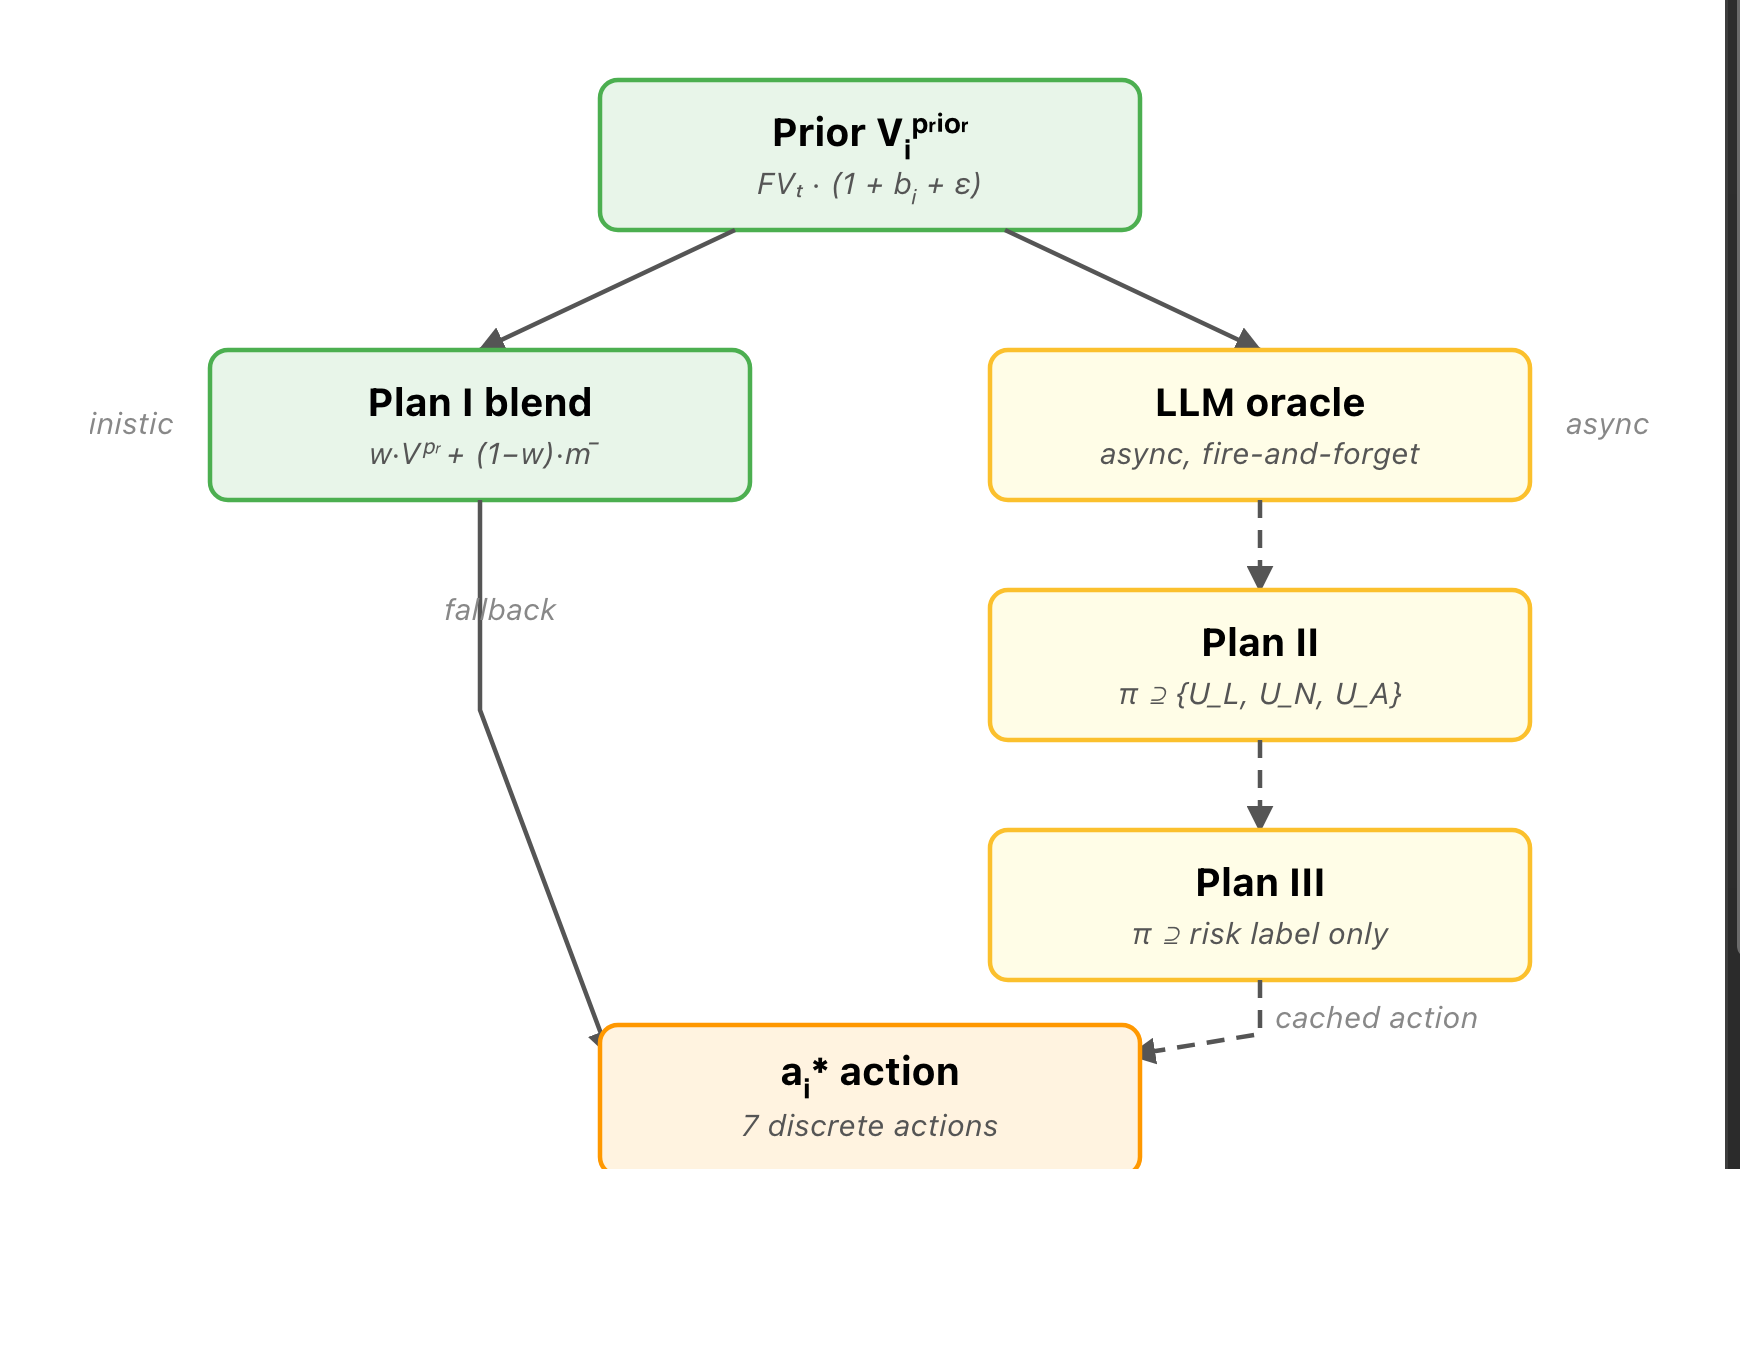
\includegraphics[width=0.75\columnwidth]{figures/llm.png}
\caption{Belief-update and action-selection data flow.
The LLM oracle (dashed) fires asynchronously at the previous period
boundary; Plan~II includes the closed-form utility expression,
Plan~III names only the risk label.  Both return a direct action
from the seven-element set.  If no reply is cached, the
agent falls through to the deterministic Plan~I blend.}
\label{fig:llm}
\end{figure}

The prompt for Plan~II encodes six fields: market structure
($T$,~$\mu$,~$\FV_t$), current state (round, period, cash,
inventory, $k_i$), the \emph{closed-form} utility expression, the
risk label, peer claims~$\msgs_i$, and mark-to-market wealth.
Plan~III deletes the utility expression; all other fields are
byte-identical.  The reply is parsed for the first decimal, clamped
to $[0,\,2\FV_1]$, and written to the belief cache.  Temperature is
set to~0.4 to allow moderate exploration while limiting pathological
outputs.

This design isolates the LLM's contribution to a single scalar per
agent per period---the posterior valuation---and routes it through the
same downstream pipeline (EU scoring, order submission, matching,
settlement) as the algorithmic baseline.  Any difference in
market-level statistics between plans is therefore attributable to
that scalar alone.
